\documentclass[UTF8,a4paper,zihao=5,fontset=fandol]{ctexart}
\usepackage[margin=21mm,top=19mm,bottom=19mm]{geometry}
\usepackage{amsmath,amssymb,graphicx,booktabs,array,caption,xcolor,adjustbox}
\usepackage[hidelinks]{hyperref}
\usepackage{fancyhdr}
\pagestyle{fancy}\fancyhf{}\fancyhead[L]{\small 机器学习课程设计}\fancyhead[R]{\small 二维变分自适应网格预测}
\fancyfoot[C]{\thepage}\setlength{\headheight}{15pt}
\setlength{\parskip}{3pt}\linespread{1.12}
\ctexset{section={format=\large\bfseries,beforeskip=8pt,afterskip=4pt},subsection={format=\normalsize\bfseries,beforeskip=6pt,afterskip=3pt}}
\captionsetup{font=small,labelformat=empty,hypcap=false,skip=3pt}
\setlength{\emergencystretch}{1em}
\begin{document}
\begin{center}{\LARGE\bfseries 直接物理网格预测与变分精修的数值实验}\end{center}

作者：\_\_\_\_\_\_\_\_　学号：\_\_\_\_\_\_\_\_　课程：机器学习课程设计


\textbf{摘要：} 本文复用已有二维变分网格教师和小型MLP，检验直接使用物理节点预测的实际价值。对30个测试实例及3个展示实例，比较规则网格、教师物理网格、原始X预测、坐标往返后的X预测和Q模型一次重建网格，并测量同一解析函数的分片线性插值误差。原始X预测与Q重建均合法，测试节点误差分别为2.19\%与2.15\%，插值精度接近，但均未优于规则网格。随后定义独立的物理坐标均匀分布/对齐能量，使用完整自动微分和单调Armijo求解。在同一物理目标下，X模型初值将平均在线时间由0.858秒降至0.702秒，终点插值RMSE较规则网格降低6.78\%。实验表明，教师拟合精度与功能精度需要分开评价，直接物理预测可作为低成本近似和优化初值。


\textbf{关键词：} 物理网格；多层感知机；变分方法；自动微分；插值误差


\section*{1 引言}

固定节点预算下的网格移动旨在将节点重新分配到需要解析的区域。变分方法以度量控制坐标分布[1]，学习方法则近似参数到网格终点的映射[2]。两者结合时，需要区分“拟合教师坐标”与“改善具体数值任务”。


已有X模型直接预测物理内部节点位移，本研究不增加训练或更换网络。新的实验是保留其原始物理输出，测量几何和独立插值指标，再探索将物理节点直接作为优化变量。物理输出无需为展示或插值先转换到计算坐标；只有进入原Q求解器时才需要那一接口。


\section*{2 数据与既有方法}

单位方形每轴12个方格，共169个节点、121个内部节点和288个三角形。固定连接及逐节点边界。复用200个真实教师，按140/30/30完整参数实例拆分，另有三个预先指定展示参数。输入为 $\mu=(c_x,c_y,A,\sigma)$，范围为 $c_x,c_y\in[0.30,0.70]$、$A\in[2,8]$、$\sigma\in[0.18,0.30]$。


原X模型与Q模型均为 $4\to64\to64\to242$ 的Tanh网络，输入和标签缩放仅使用训练集。保留原X权重和第三轮预先固定的Q权重；不重新选择模型，不产生教师样本。X标签为物理位移，Q标签为计算位移，二者数值意义不同。


原求解器在固定物理网格 $X_0$ 上冻结度量，以计算节点Q为变量：


\[
I_h(Q;\mu)=\sum_K |K(X_0)|\operatorname{tr}
\left(B_K(Q)E_K(X_0)^{-1}M_K^{-1}E_K(X_0)^{-T}B_K(Q)^T\right).
\]

其输出物理网格为 $X_T=R(Q_T)$。原始X预测为P，仅物理退缩得到 $P_{safe}$；旧转换分支还执行 $R(C(P_{safe}))$。本实验分别保存这些对象，不把物理X直接代入旧Q能量。



\newpage

\section*{3 独立的物理坐标变分目标}

固定参考三角形的边矩阵记为 $\widehat E_K$，物理边矩阵为 $E_K(X)$。定义物理到参考的逆Jacobian


\[
J_K(X)=\widehat E_KE_K(X)^{-1},\qquad
M_K(X)=m_K(X)I_2,\qquad
m_K(X)=1+A\exp\left(-\frac{|x_K(X)-c|^2}{\sigma^2}\right).
\]

其中 $x_K(X)$ 为当前物理重心。采用文献[1]式(11)的泛函族，取 $d=2,p=2,\theta=1/3$，在每个物理单元做重心求积：


\[
E_{\rm phys}(X)=\sum_K |K(X)|m_K(X)\left[
\frac13\left(\frac{\|J_K(X)\|_F^2}{m_K(X)}\right)^2+
\frac43\left(\frac{\det J_K(X)}{m_K(X)}\right)^2\right].
\]

面积、Jacobian及度量均依赖X，不能使用原冻结物理网格上的Q梯度。用PyTorch float64对整个离散表达式自动微分，保留面积、逆矩阵和重心度量的全部导数，最后将边界梯度置零。对规则和变形训练实例各取两个固定随机方向，中心差分步长 $10^{-6}$，方向导数差异通过 $10^{-7}$ 的归一化检查。


正面积下能量为正，且 $1\le m\le9$。局部缩放时逆Jacobian与面积共同作用，p=2的项提供面积分配惩罚；退化单元的逆Jacobian增长不能由有界m抵消。坐标和度量在单位方形上无量纲。连续泛函的性质不自动给出本离散问题的唯一性，本文只验证实现的导数、几何、下降与数值停止条件。


\subsection*{3.1 相同物理目标的求解}

规则初值与原X模型物理初值共用同一能量与求解程序。采用投影负梯度方向，BB谱步长提议[3]为


\[
\alpha_{BB}=\frac{s^Ts}{s^Ty},\quad
s=X_k-X_{k-1},\quad y=g_k-g_{k-1}.
\]

曲率非正则取0.1，初始提议0.1，提议限制 $[10^{-8},1]$。Armijo系数 $10^{-4}$、退缩因子1/2，仅接受有限、区域内、边界固定、全部有向面积大于 $10^{-10}$ 且真实充分下降的候选。停止条件为 $\|g\|_2\le10^{-5}$，上限3000次接受迭代、30000次能量评价。梯度求值的前向计算也计入能量评价。


\subsection*{3.2 几何及独立功能指标}

使用最小有向面积、翻转数、最小角，以及 $q_K=4\sqrt3|K|/\sum_{e\subset K}|e|^2$ 评价形状；q越接近1越好。所有网格在相同160×160中点采样上插值


\[
u_\mu(x,y)=\exp\left(-\frac{(x-c_x)^2+(y-c_y)^2}{\sigma^2}\right),\quad
e_{\rm int}=\sqrt{\frac1N\sum_{j=1}^N\left(u_h(z_j)-u_\mu(z_j)\right)^2}.
\]

节点值取解析场真值，使用同一三角连接上的分片线性插值。该采样RMSE独立于教师坐标标签，是插值实验而非PDE解误差。



\newpage

\section*{4 直接使用物理预测的测试结果}

表1为30个独立测试实例均值；最小角与RMSE后为实例间样本标准差。节点误差分母为教师内部物理移动量 $\|X_T-X_0\|_\mathcal I$，不移动误差为1。q为每张网格最差单元质量的均值。


\begin{center}\small\begin{adjustbox}{max width=\linewidth}\begin{tabular}{lllll}\toprule
物理网格 & 节点误差/\% & 最小角/度 & 最差质量q & RMSE×1000 \\
\midrule
规则网格 & 100.000 & 45.00 ± 0.00 & 0.866 & 10.028 ± 1.424 \\
旧Q教师物理网格 & 0.000 & 24.36 ± 2.80 & 0.601 & 10.326 ± 1.634 \\
X模型直接输出 & 2.195 & 24.38 ± 2.57 & 0.604 & 10.280 ± 1.563 \\
X模型经坐标往返 & 6.280 & 25.92 ± 2.53 & 0.622 & 9.635 ± 1.287 \\
Q模型一次重建 & 2.147 & 24.31 ± 2.58 & 0.601 & 10.285 ± 1.572 \\
\bottomrule\end{tabular}\end{adjustbox}\end{center}

\begin{center}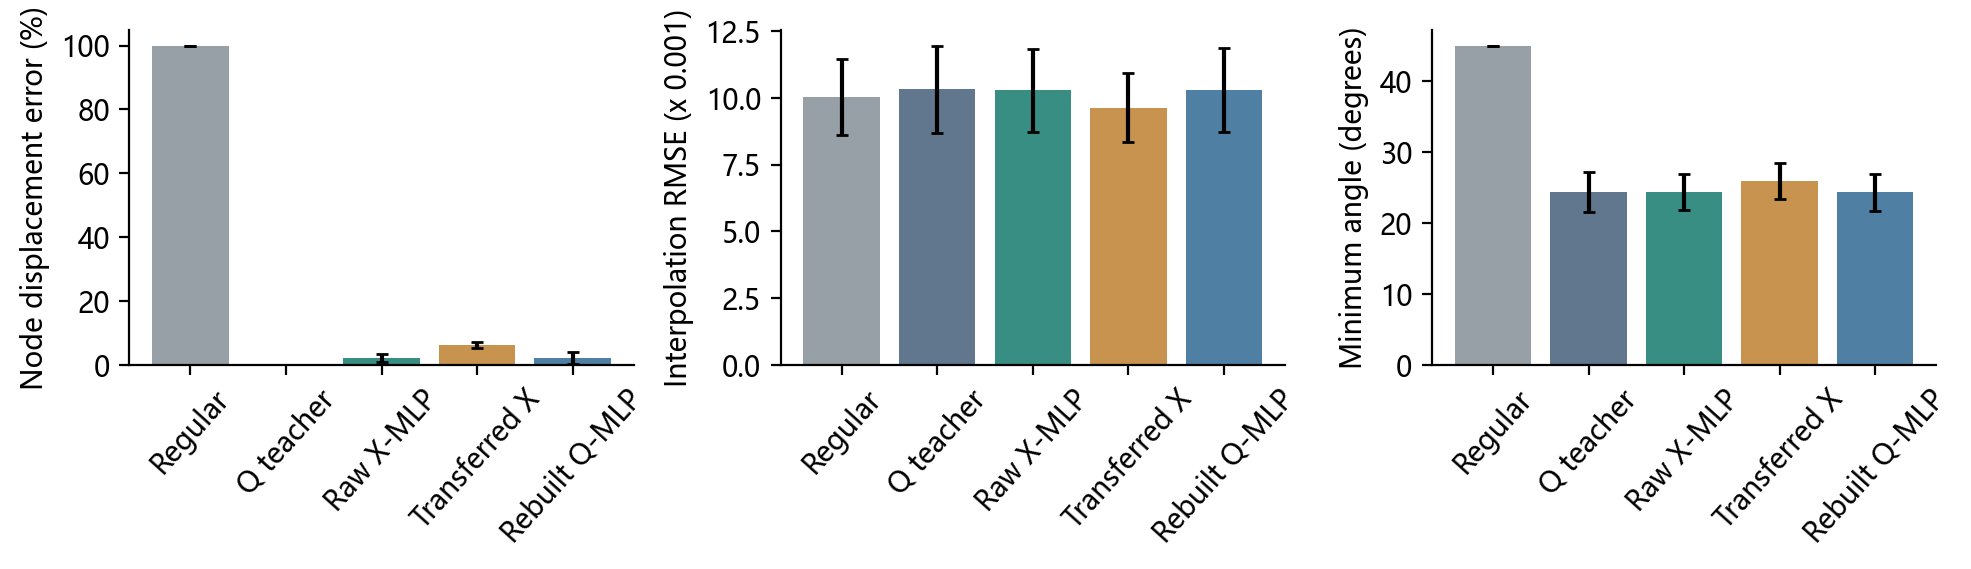
\includegraphics[width=\linewidth]{../results/A_comparison.png}\captionof{figure}{图1　节点误差、采样插值RMSE与最小角。误差棒为30个实例间的样本标准差。}\end{center}

直接X预测在33个未见实例上均合法且无需退缩，测试节点误差为2.19\%，与Q模型的2.15\%接近。两者插值RMSE分别为0.010280和0.010285；直接X相对规则网格的平均RMSE增加2.52\%。


实验A共165个状态均合法，翻转数为零，原始X预测的33个实例均不需要位移退缩。X与Q预测的最小角和最差单元质量接近。规则网格的形状质量最高，但形状与节点分配共同决定插值表现，单独的几何质量不是充分指标。


旧教师的平均插值RMSE也高于规则网格，说明该教师在这一解析场和节点预算下不是插值最优网格。度量根据高斯函数值设定，并未按插值误差最小化构造；因此更接近教师不必然降低RMSE。经坐标往返的X输出虽然节点误差更大，其RMSE却较低，这是评价目标不同的实际例子。


表2为模型预加载后的生成时间。固定拓扑接口预建，包含输入归一化与推理、物理合法性检查，Q分支还含一次R重建；旧转移分支含C/R。三分支交替顺序各重复三次，误差评估不计时。


\begin{center}\small\begin{adjustbox}{max width=\linewidth}\begin{tabular}{llll}\toprule
预测分支 & 推理/ms & 检查或转换/ms & 完整生成/ms \\
\midrule
X模型直接输出 & 0.288 & 0.253 & 0.542 \\
X模型经坐标往返 & 0.241 & 3.833 & 4.074 \\
Q模型一次重建 & 0.306 & 1.908 & 2.215 \\
\bottomrule\end{tabular}\end{adjustbox}\end{center}

三个展示实例用320×320采样复核，所有五状态RMSE的最大相对变化为0.0268\%。较密采样支持本次误差量级判断，但不把X与Q之间极小的均值差解释为稳定精度优势。



\newpage

\section*{5 三个代表性算例}

\subsection*{5.1 中心加密}

\begin{center}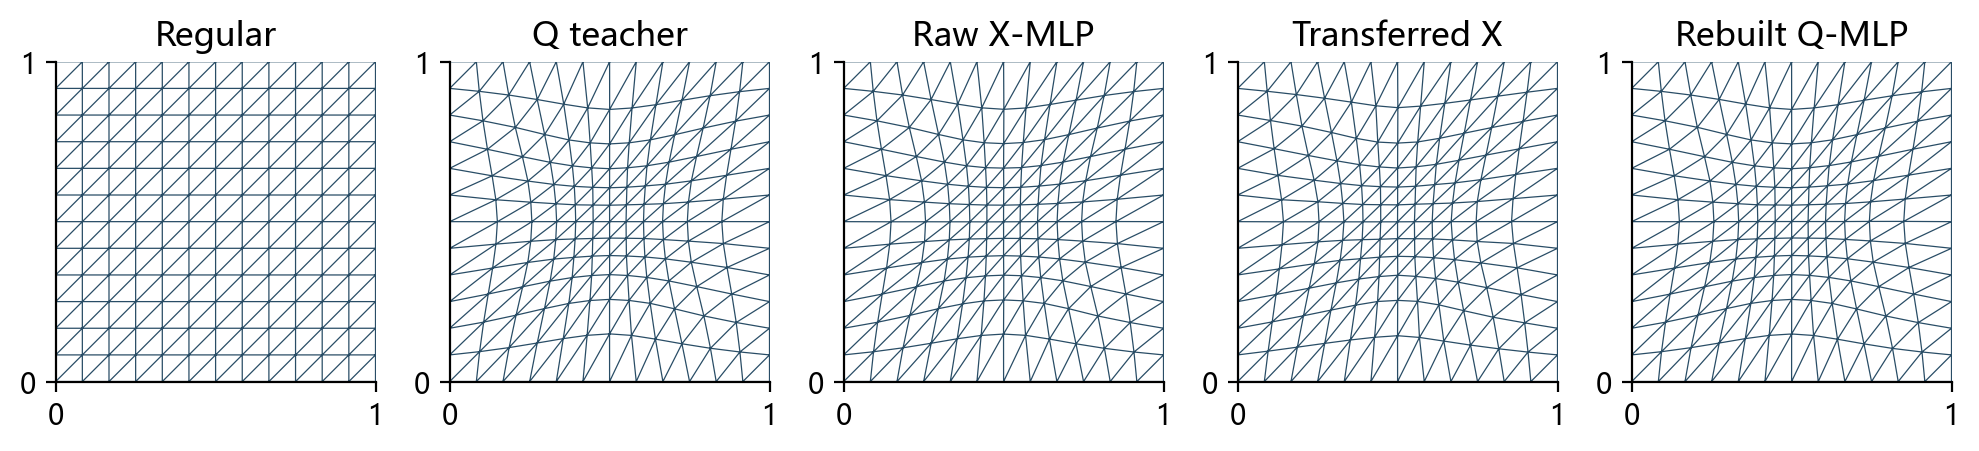
\includegraphics[width=\linewidth]{../results/case_center.png}\captionof{figure}{图2　中心度量：规则、教师、原始X、转换X和Q重建物理网格。}\end{center}

参数为 $\mu=(0.50,0.50,5.0,0.24)$。所有分支使用同一节点编号、边界与连接，五张图的范围一致。原始X的物理输出未经计算坐标往返。


\subsection*{5.2 加密中心偏移}

\begin{center}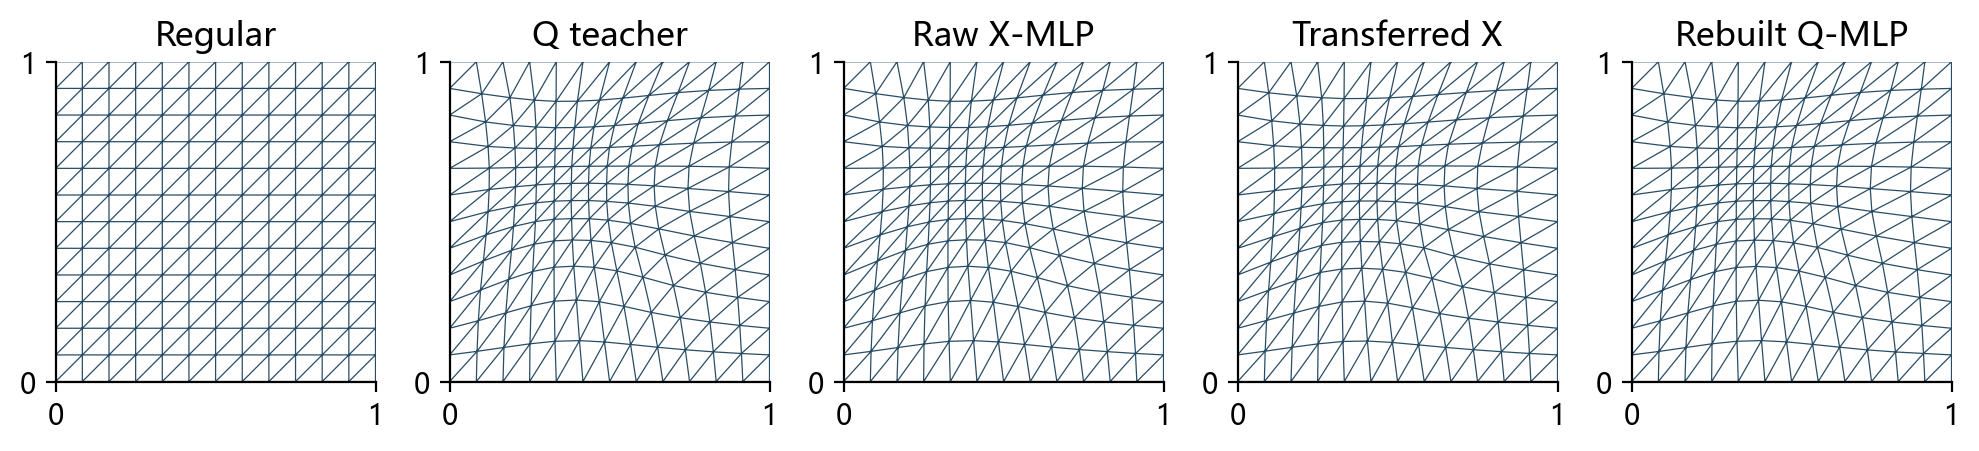
\includegraphics[width=\linewidth]{../results/case_shifted.png}\captionof{figure}{图3　偏心度量的五状态比较。}\end{center}

参数为 $\mu=(0.36,0.64,5.0,0.24)$，考察区间内部加密位置移动。模型不为此例单独拟合。


\subsection*{5.3 强度及宽度变化}

\begin{center}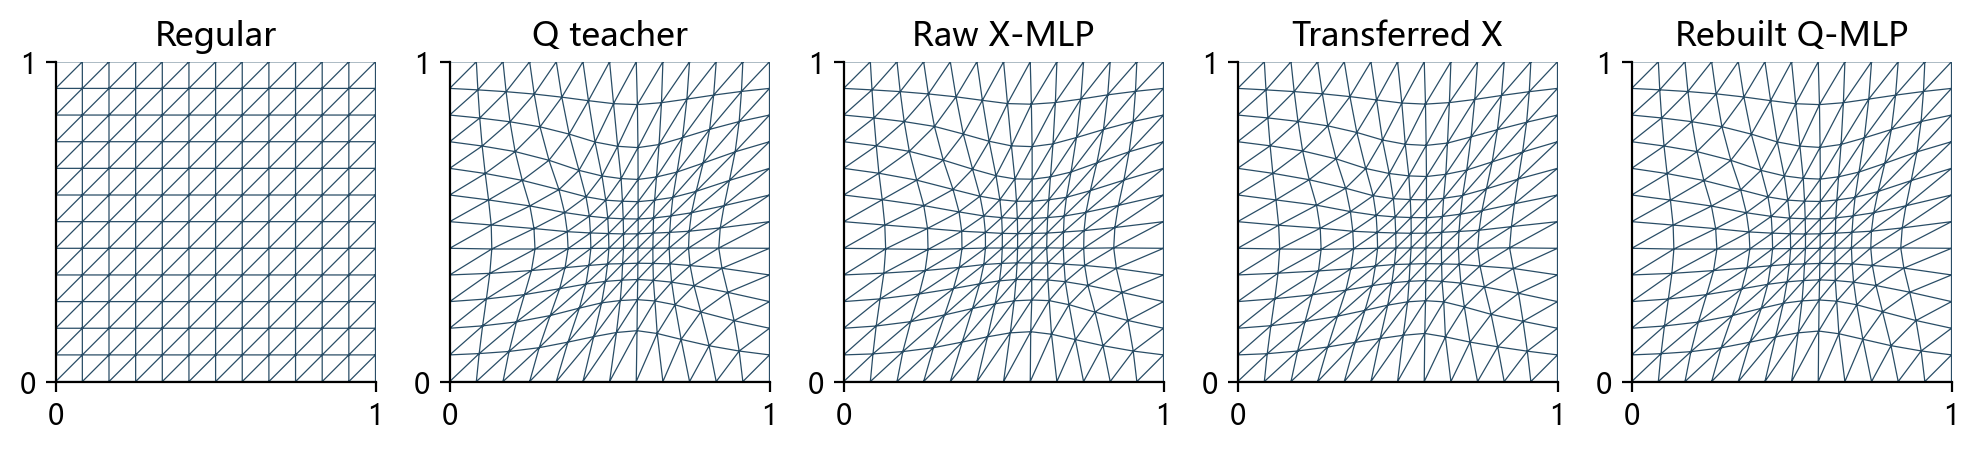
\includegraphics[width=\linewidth]{../results/case_strength.png}\captionof{figure}{图4　较强、较窄高斯度量的五状态比较。}\end{center}

参数为 $\mu=(0.58,0.43,7.5,0.19)$。下表最后一列仅比较同一物理目标的两种初值。


\begin{center}\small\begin{adjustbox}{max width=\linewidth}\begin{tabular}{llllll}\toprule
算例 & 规则RMSE & 原始X RMSE & Q重建RMSE & 物理精修RMSE & 同目标加速 \\
\midrule
center & 0.00971 & 0.01080 & 0.01085 & 0.00944 & 0.87 \\
shifted & 0.00959 & 0.01007 & 0.01009 & 0.00922 & 1.34 \\
strength & 0.01211 & 0.01288 & 0.01297 & 0.01122 & 1.27 \\
\bottomrule\end{tabular}\end{adjustbox}\end{center}


\newpage

\section*{6 物理坐标直接优化的结果}

实验B的66组终点全部合法并达到共同物理梯度阈值，198次重复运行均收敛。下表为测试集均值，时间后的标准差为实例间差异；单实例三次计时的标准差保存在逐实例CSV。


\begin{center}\small\begin{adjustbox}{max width=\linewidth}\begin{tabular}{lllll}\toprule
物理目标的初值 & 接受迭代 & 能量评价 & 在线时间/s & 收敛数 \\
\midrule
规则网格 & 205.1 & 591.6 & 0.858 ± 0.294 & 30/30 \\
X模型输出 & 167.1 & 487.8 & 0.702 ± 0.262 & 30/30 \\
\bottomrule\end{tabular}\end{adjustbox}\end{center}

\begin{center}\small\begin{adjustbox}{max width=\linewidth}\begin{tabular}{lllll}\toprule
初值 & 初始E\_phys & 终点E\_phys & 终点梯度范数 & 终点插值RMSE \\
\midrule
规则网格 & 1.91182496 & 1.69650846 & 8.84e-06 & 0.009347 \\
X模型输出 & 1.70722083 & 1.69650846 & 8.88e-06 & 0.009347 \\
\bottomrule\end{tabular}\end{adjustbox}\end{center}

\begin{center}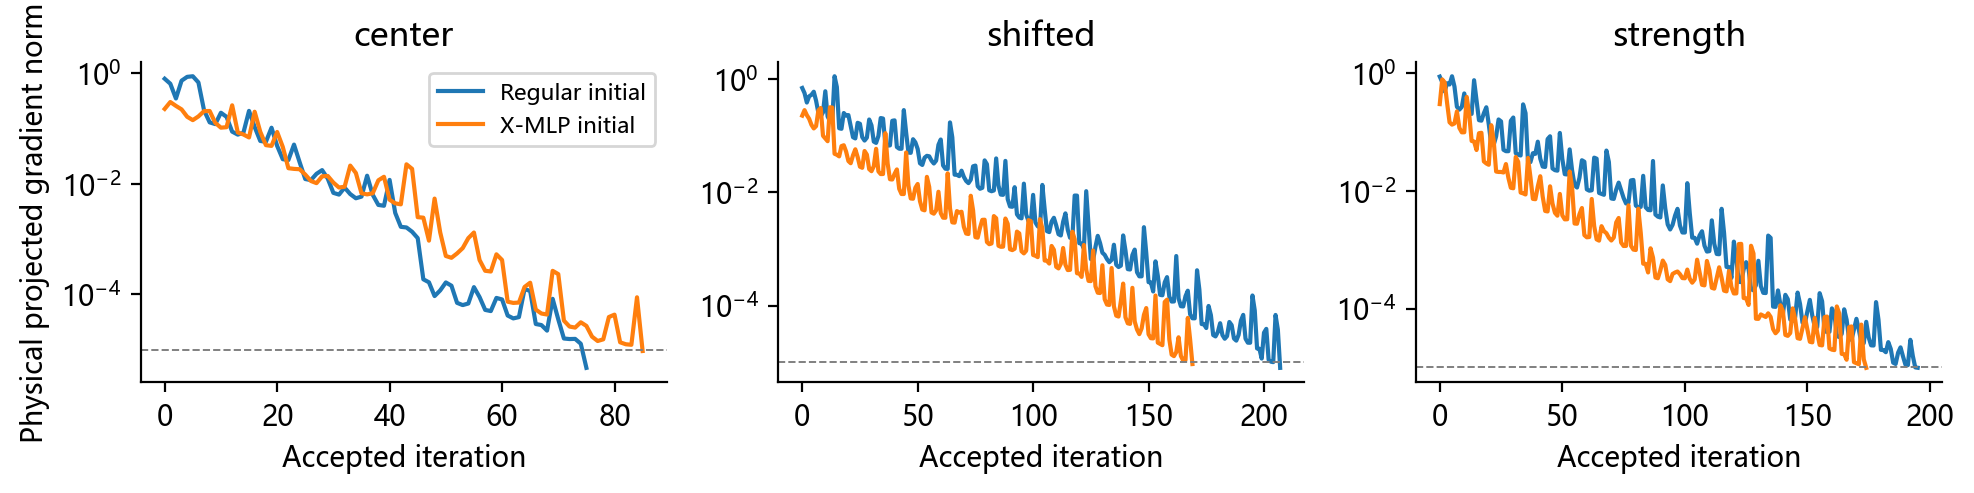
\includegraphics[width=\linewidth]{../results/B_convergence.png}\captionof{figure}{图5　三个展示实例的物理能量投影梯度轨迹；虚线为共同停止阈值。}\end{center}

\begin{center}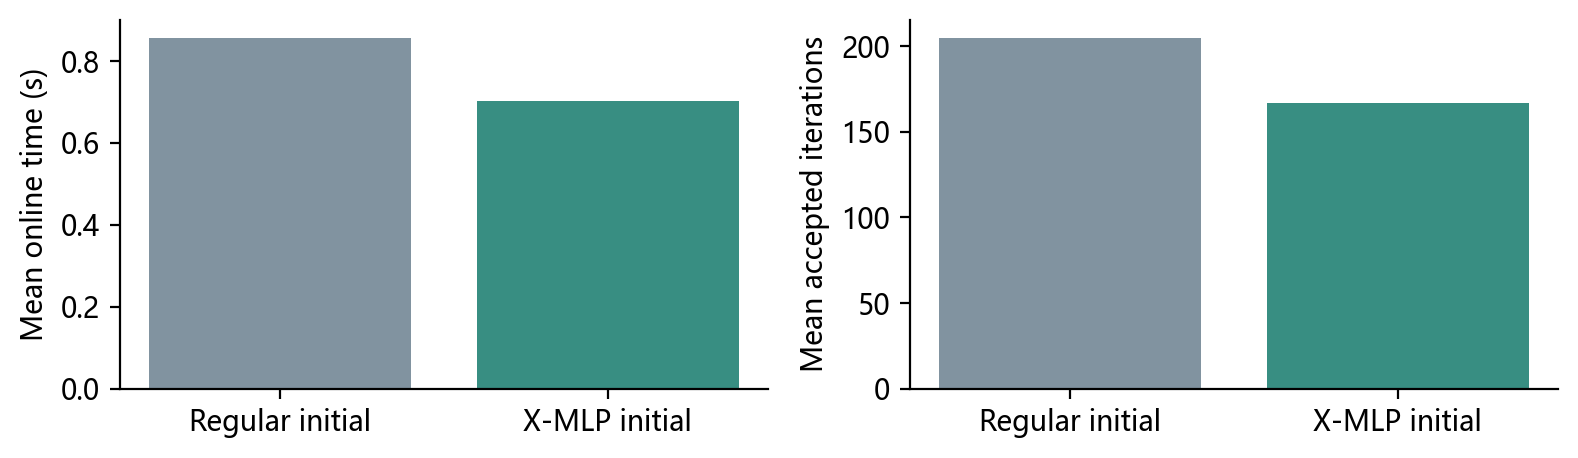
\includegraphics[width=\linewidth]{../results/B_cost.png}\captionof{figure}{图6　同一物理目标下的完整在线时间与接受迭代数。}\end{center}

独立物理目标下，规则初值与X模型初值均达到共同梯度阈值。平均接受迭代由205.1降至167.1，完整在线时间由0.858秒降至0.702秒，均值比加速1.22倍。物理精修后RMSE为0.009347，较规则网格降低6.78\%。


30个测试实例中，MLP初值在26个实例上耗时较短。两种初值终点的最大相对能量差为3.99e-11，以规则物理优化终点移动量归一化的最大节点距离为9.02e-05，本次未观察到不同终点导致的明显精度差异。物理目标终点相对旧Q教师约16.95\%的坐标差是不同目标产生的结果，不能解释为相同教师精修失败。



\newpage

\section*{7 结果解释与课程设计选择}

\begin{center}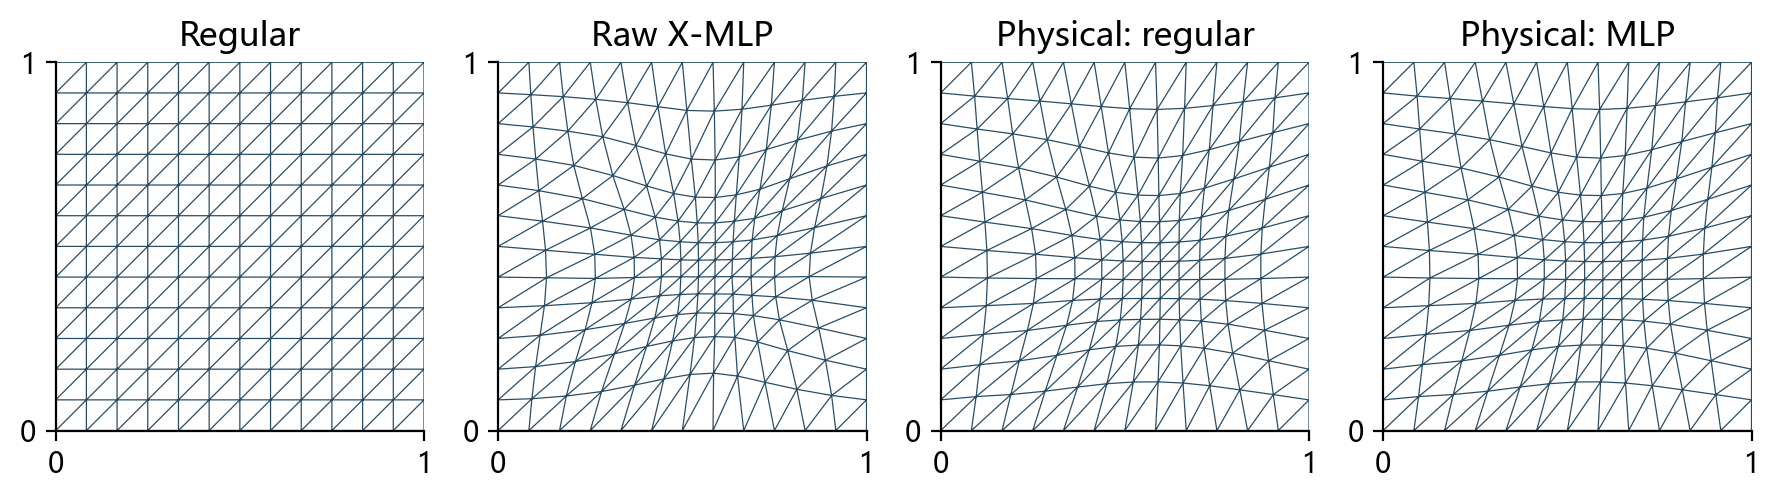
\includegraphics[width=\linewidth]{../results/B_mesh.png}\captionof{figure}{图7　较强度量下，规则和原始X预测与两个物理优化终点。}\end{center}

\subsection*{7.1 直接物理输出的价值}

直接X输出以约0.542毫秒完成预测和检查，保留了约2\%的教师位移拟合精度，省去离散往返。与Q模型一次重建的插值误差和几何质量基本相同，因而对快速给出教师近似具有价值。其平均插值RMSE略高于规则网格，不能据此宣称直接预测本身改善了插值任务。


独立物理能量在本问题族上可求导、可下降并达到共同阈值。MLP初值减少约18.5\%的接受迭代、约18.1\%的在线时间。两种初值都能获得相近终点，因此MLP的主要作用是减少达到终点的成本，而非创造传统方法无法获得的网格。


课程设计可保留“直接物理预测作为廉价近似与物理优化初值”的方案，以独立插值评测和同目标精修为核心。单独的原始X预测适合快速逼近教师，本次插值指标不支持把它作为无需后处理的最终优胜网格；物理精修的收益温和，需计入离线成本。


\subsection*{7.2 离线成本与限制}

既有203个教师求解累计227.38秒，X模型训练26.65秒，本轮没有新增教师或训练。若这些成本专为部署产生，按本次同目标平均节省估算，约需1634次同分布调用摊平；若教师已有其他用途，可单列新增成本，不能将离线阶段视为免费。


本实验固定拓扑、分辨率、区域与单高斯参数范围，未涉及PDE误差或分布外泛化。度量不是针对本插值任务最优设计，物理重心求积目标也不保证全局唯一极小点。I\_h与E\_phys是不同离散目标，能量大小、梯度阈值和时间不能跨目标作同精度加速比较。时间受本机负载影响，模型及固定拓扑接口预加载，指标与磁盘操作排除；三次重复均保留。网页构建检查与实际浏览器验收状态见README。


\section*{8 结论}

直接使用原始物理预测避免多余坐标往返，在本测试集上具有合法、廉价且接近教师的特点，但对指定解析场未优于规则网格。使用独立的物理坐标能量精修可改善本次插值指标，X模型作为同目标优化初值取得1.22倍的温和加速。课程设计的可靠结论是同时检验教师拟合、几何与独立功能指标，并将初值收益限定在同一优化目标内。


\section*{参考文献}

\begin{sloppypar}[1] Huang W., Kamenski L., Russell R. D. A comparative numerical study of meshing functionals for variational mesh adaptation. Journal of Mathematics Study, 2015, 48(2):168–186. DOI:10.4208/jms.v48n2.15.04. \href{https://arxiv.org/abs/1503.04709}{论文原文}。\end{sloppypar}


\begin{sloppypar}[2] Song W., Zhang M., Wallwork J. G., et al. M2N: Mesh Movement Networks for PDE Solvers. Advances in Neural Information Processing Systems, 35, 2022. \href{https://proceedings.neurips.cc/paper\_files/paper/2022/hash/2f88d8061f12abae9d14d376fd69c933-Abstract-Conference.html}{会议原文}。\end{sloppypar}


\begin{sloppypar}[3] Barzilai J., Borwein J. M. Two-Point Step Size Gradient Methods. IMA Journal of Numerical Analysis, 1988, 8(1):141–148. DOI:10.1093/imanum/8.1.141. \href{https://doi.org/10.1093/imanum/8.1.141}{期刊入口}。\end{sloppypar}

\end{document}